% Included from both -slides and -handout versions.
\usetheme{metropolis}

\usepackage[english]{babel}
\usepackage[latin1]{inputenc}
\usepackage{graphicx}
\usepackage{times}
\usepackage[T1]{fontenc}
\usepackage{fancyvrb}
\usepackage{listings}
\begin{document}
\lstset{language=C, escapeinside={(*@}{@*)}, numbers=left,
  basicstyle=\tiny, showspaces=false, showtabs=false}

\title{Introduction to Operating Systems}
\subtitle{Through tracing, analysis, and experimentation}
%\institute{University of Cambridge}
\author{George V. Neville-Neil}
%\author{Dr Robert N. M. Watson}
\date{1 August 2016}

\begin{frame}
  \titlepage
\end{frame}

\section{Communcation}
\label{sec:communication}

\section{Inter-Process Communication}
\label{sec:ipc}

\begin{frame}
  \frametitle{Goals of IPC}
  \begin{itemize}
  \item Data Sharing
  \item Signaling events
  \item Control of multiple processes
  \end{itemize}
\end{frame}

\begin{frame}
  \frametitle{Mechanisms}
  \begin{itemize}
  \item Shared files
  \item Semaphores and Mutexes
  \item Signals
  \end{itemize}
\end{frame}

\begin{frame}
  \frametitle{History}
  \begin{itemize}
  \item 
  \item 
  \item 
  \end{itemize}
\end{frame}

\begin{frame}
  \frametitle{Relationship to Networking}
  \begin{itemize}
  \item 
  \item 
  \item 
  \end{itemize}
\end{frame}

\begin{frame}
  \frametitle{Signals}
  \begin{itemize}
  \item 
  \item 
  \item 
  \end{itemize}
\end{frame}

\begin{frame}
  \frametitle{}
  \begin{itemize}
  \item 
  \item 
  \item 
  \end{itemize}
\end{frame}

\begin{frame}
  \frametitle{Pipes}
  \begin{itemize}
  \item 
  \item 
  \item 
  \end{itemize}
\end{frame}

\begin{frame}
  \frametitle{}
  \begin{itemize}
  \item 
  \item 
  \item 
  \end{itemize}
\end{frame}

\begin{frame}
  \frametitle{}
  \begin{itemize}
  \item 
  \item 
  \item 
  \end{itemize}
\end{frame}

\begin{frame}
  \frametitle{}
  \begin{itemize}
  \item 
  \item 
  \item 
  \end{itemize}
\end{frame}

\begin{frame}
  \frametitle{}
  \begin{itemize}
  \item 
  \item 
  \item 
  \end{itemize}
\end{frame}

\begin{frame}
  \frametitle{}
  \begin{itemize}
  \item 
  \item 
  \item 
  \end{itemize}
\end{frame}

\begin{frame}
  \frametitle{}
  \begin{itemize}
  \item 
  \item 
  \item 
  \end{itemize}
\end{frame}

\begin{frame}
  \frametitle{}
  \begin{itemize}
  \item 
  \item 
  \item 
  \end{itemize}
\end{frame}

\begin{frame}
  \frametitle{}
  \begin{itemize}
  \item 
  \item 
  \item 
  \end{itemize}
\end{frame}

\begin{frame}
  \frametitle{}
  \begin{itemize}
  \item 
  \item 
  \item 
  \end{itemize}
\end{frame}


\section{Internetworked Communication}
\label{sec:internet}

begin{frame}
  \frametitle{Networking and FreeBSD}
  \begin{itemize}
  \item Everyone's TCP/IP Stack
  \item IPv4, IPv6, UDP, TCP, SCTP
  \item Various drivers
  \item Multiple firewalls
  \end{itemize}
\end{frame}

\begin{frame}
  \frametitle{The User Program View}
  \begin{itemize}
  \item User programs use sockets
  \item Network programs follow UNIX model
  \item Flexible interfaces for different protocols
  \end{itemize}
\end{frame}

\begin{frame}
  \frametitle{Sockets}
  \begin{itemize}
  \item Main programmer interface to networking
  \item Generic API
  \item Attempts to support read/write semantics
  \end{itemize}
\end{frame}

\begin{frame}[fragile]
  \frametitle{Looking Directly at Sockets}
\begin{verbatim}
# Count sockets by family

# Count sockets by type

# Count sockets by protocol
\end{verbatim}  
\end{frame}

\begin{frame}
  \frametitle{Network Lab (Sockets Exercises)}
  \begin{itemize}
  \item Count socket calls by domain, type and protocol
  \item Show programs accepting connections
  \item Show programs initiating connections
  \item Write a D script to trace a single socket with the test program
  \end{itemize}
\end{frame}

\begin{frame}
  \frametitle{Network Stack}
\end{frame}

\begin{frame}
  \frametitle{Network Stack Overview}
\centering
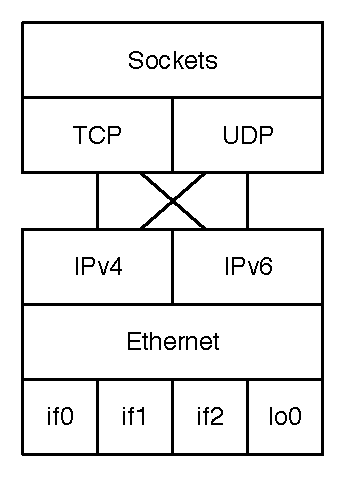
\includegraphics{../figures/tcpipstack}
\end{frame}

\begin{frame}
\centering
  \frametitle{Inbound Layer Transitions}
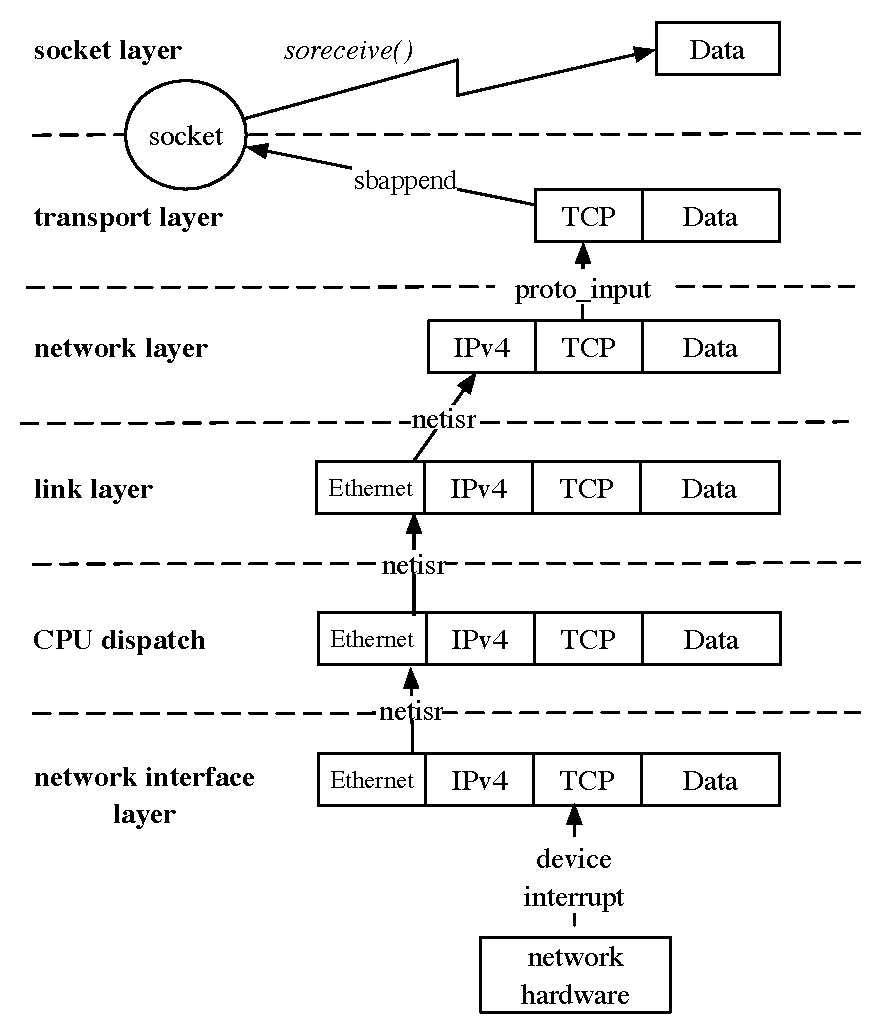
\includegraphics[width=0.5\textwidth]{../figures/inbound}
\end{frame}

\begin{frame}[fragile]
  \frametitle{UDP}
  \begin{itemize}
  \item Simplest transport protocol
  \item No states to maintain
  \item Data is sent immediately
  \item Supports multicast
  \item Only probes are \verb+send+ and \verb+receive+
  \end{itemize}
\end{frame}

\begin{frame}[fragile]
  \frametitle{UDP Send and Receive}
  \begin{itemize}
  \item \verb|udptrack|
  \end{itemize}
\end{frame}

\begin{frame}
  \frametitle{TCP}
  \begin{itemize}
  \item Transmission Control Protocol
  \item Stream based
  \item In order delivery
  \item Maintains the illusion of a byte stream
  \end{itemize}
\end{frame}

\begin{frame}[fragile]
  \frametitle{TCP Connections}
  \begin{itemize}
  \item \verb|tcpconn|
  \end{itemize}
\end{frame}

\begin{frame}[fragile]
  \frametitle{TCP State Machine}
  \begin{itemize}
  \item \verb|tcpstate|
  \end{itemize}
\end{frame}

\begin{frame}[fragile]
  \frametitle{Tracking More of TCP}
  \begin{itemize}
  \item \verb|tcptrack|
  \end{itemize}
\end{frame}

\begin{frame}[fragile]
  \frametitle{Network Protocol Lab Exercises}
  \begin{itemize}
  \item Add IP source and destination information to \verb+tcpstate+
  \item Add support for \verb+send+ and \verb+receive+ calls to \verb+tcptrack+
  \item Show the congestion window for a single connection over time
  \end{itemize}
\end{frame}

\end{document}

%%% Local Variables:
%%% mode: latex
%%% TeX-master: "lecture1-intro"
%%% End:
